%%%%%%%%%%%%%%%%%%%%%%%%%%% Supplement %%%%%%%%%%%%%%%%%%%%%%%%%%%%%%%%%%%%%%%%%%%%%

\section{Supplements}

\subsection{Gene expression in genetic variants}

\FloatBarrier

\begin{figure}
	\centering
	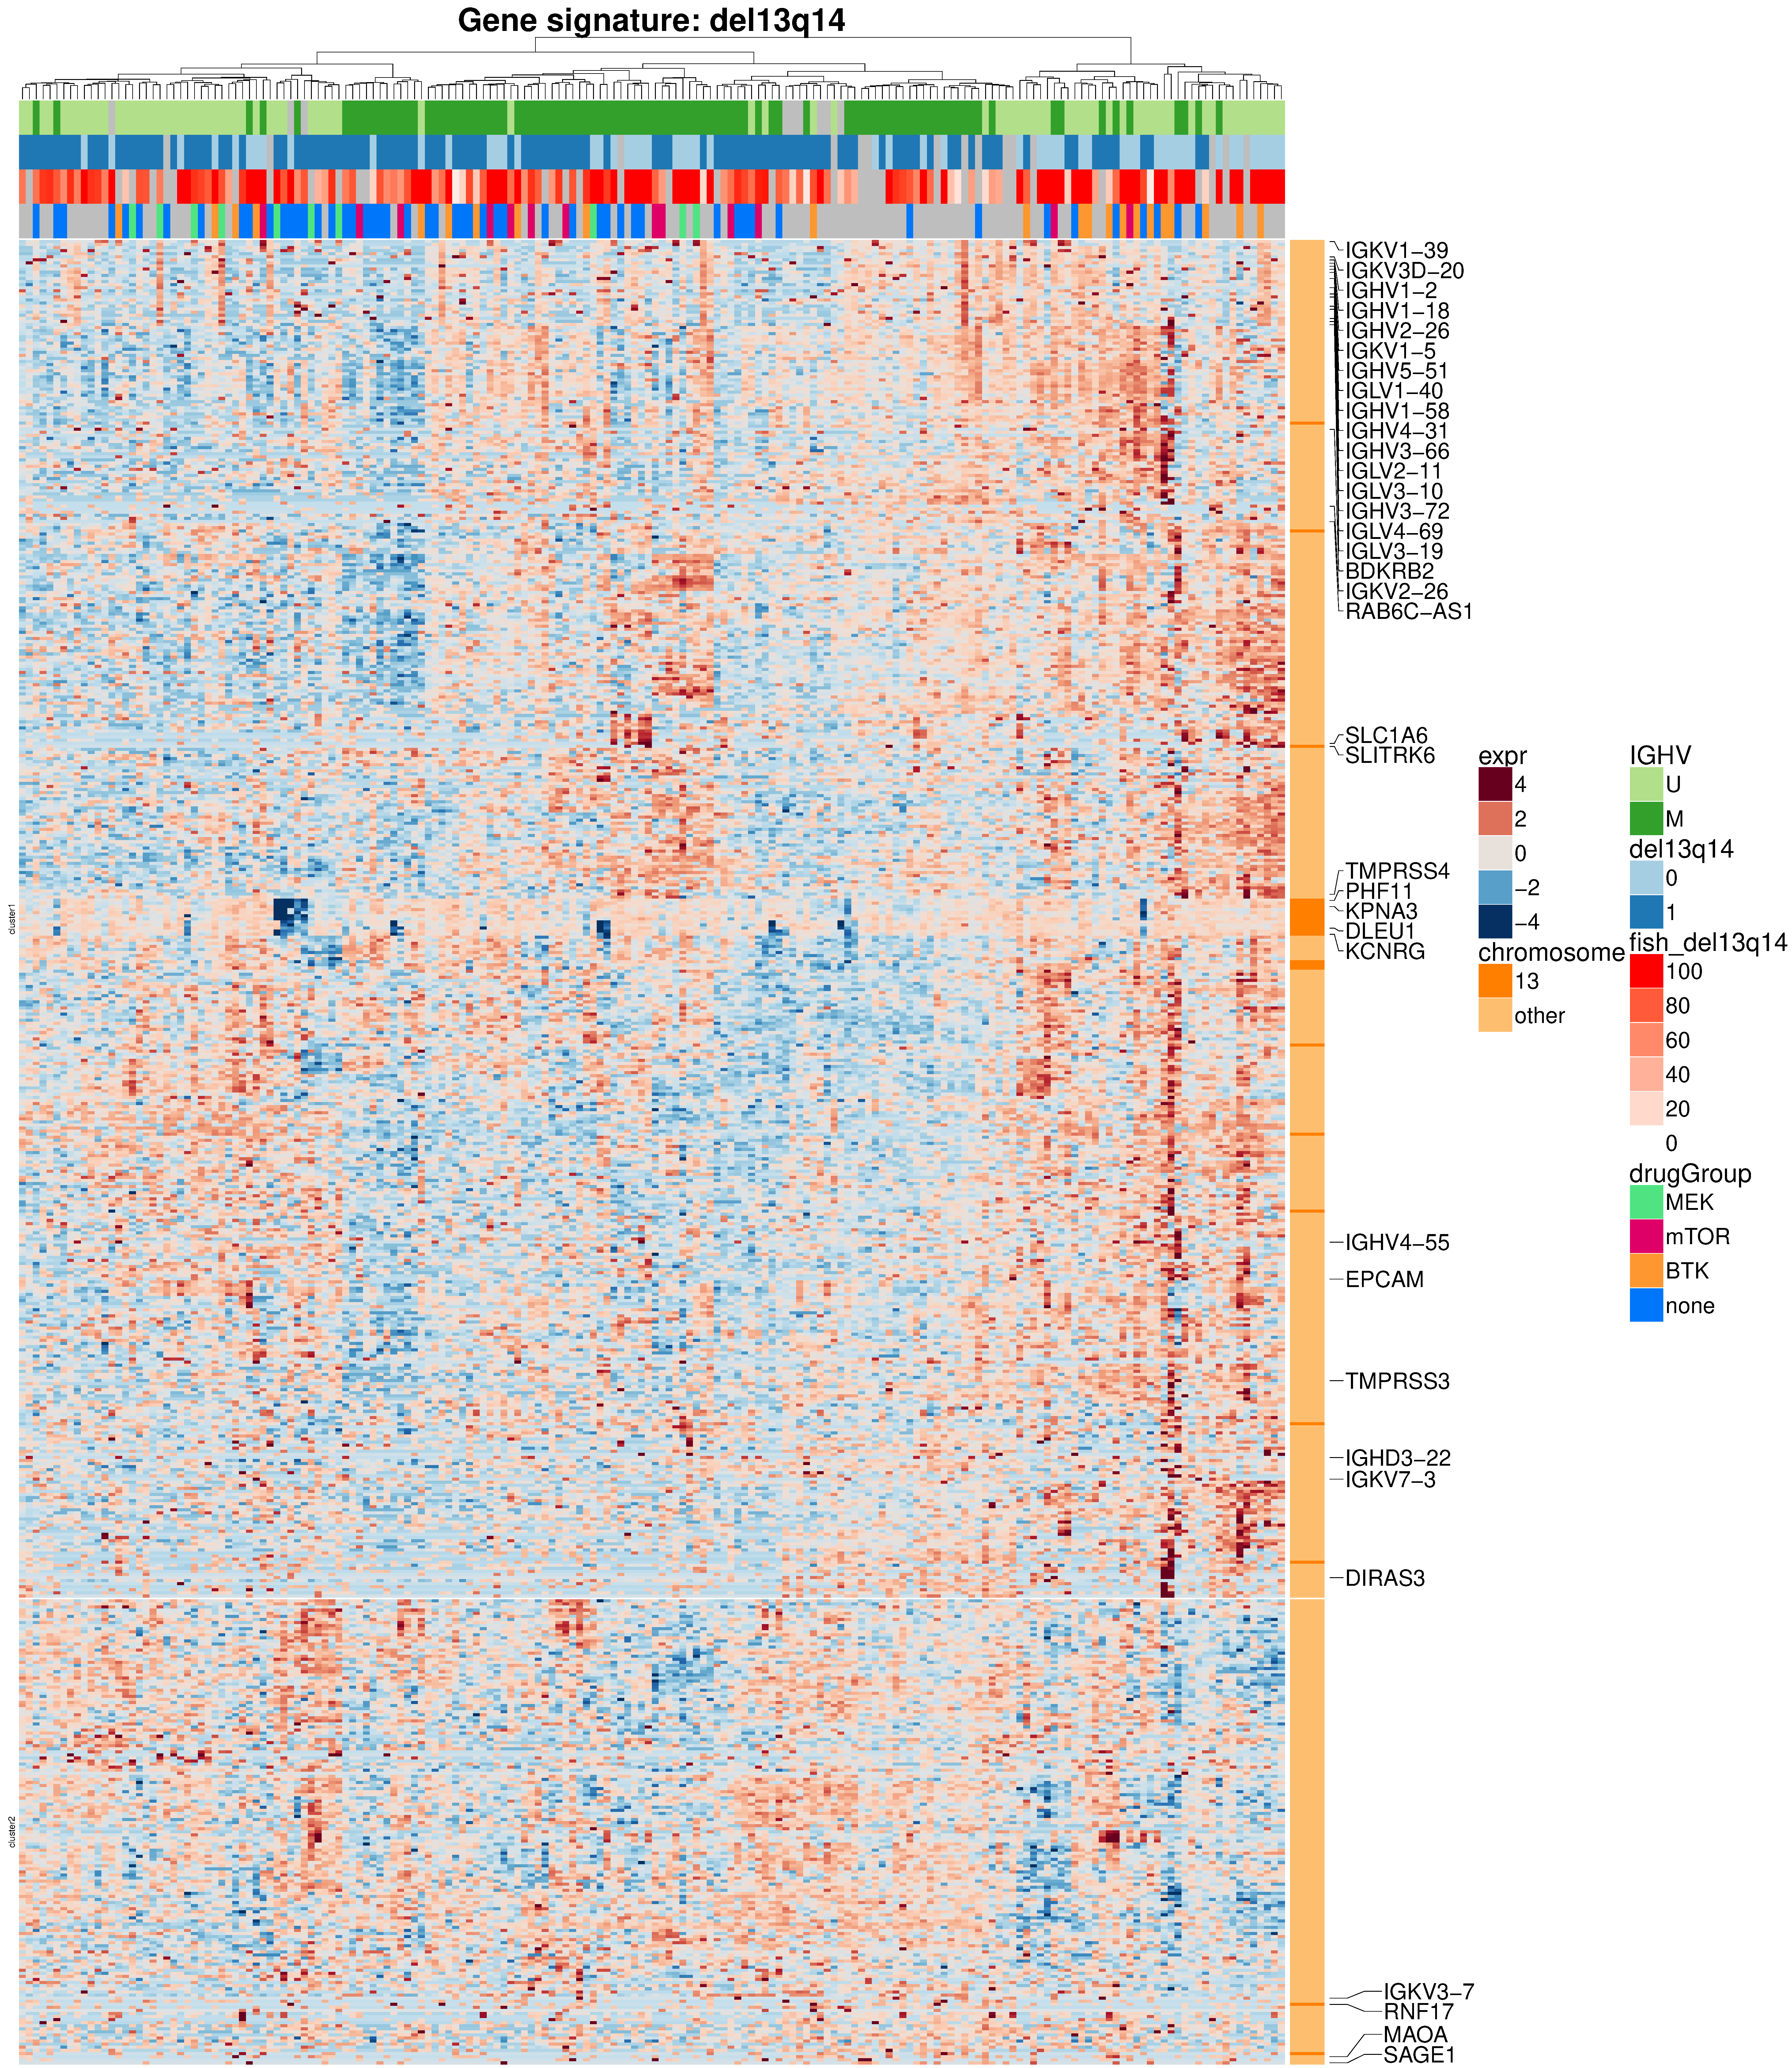
\includegraphics[width=\columnwidth]{./Figures/gene_exprDel13q14_gsea_Kegg.pdf}
	\caption{\textbf{Gene expression in Del13q14:} Del13q14 patients do not cluster based on differentially expressed genes. The percentage of deletion or drug response groups does not show any pattern either. We find DLEU1 and some further genes located within the deletion among the differentially expressed genes.}
	\label{fig:gene_exprdel13q14_gsea_kegg}
\end{figure}

\begin{figure}
	\centering
	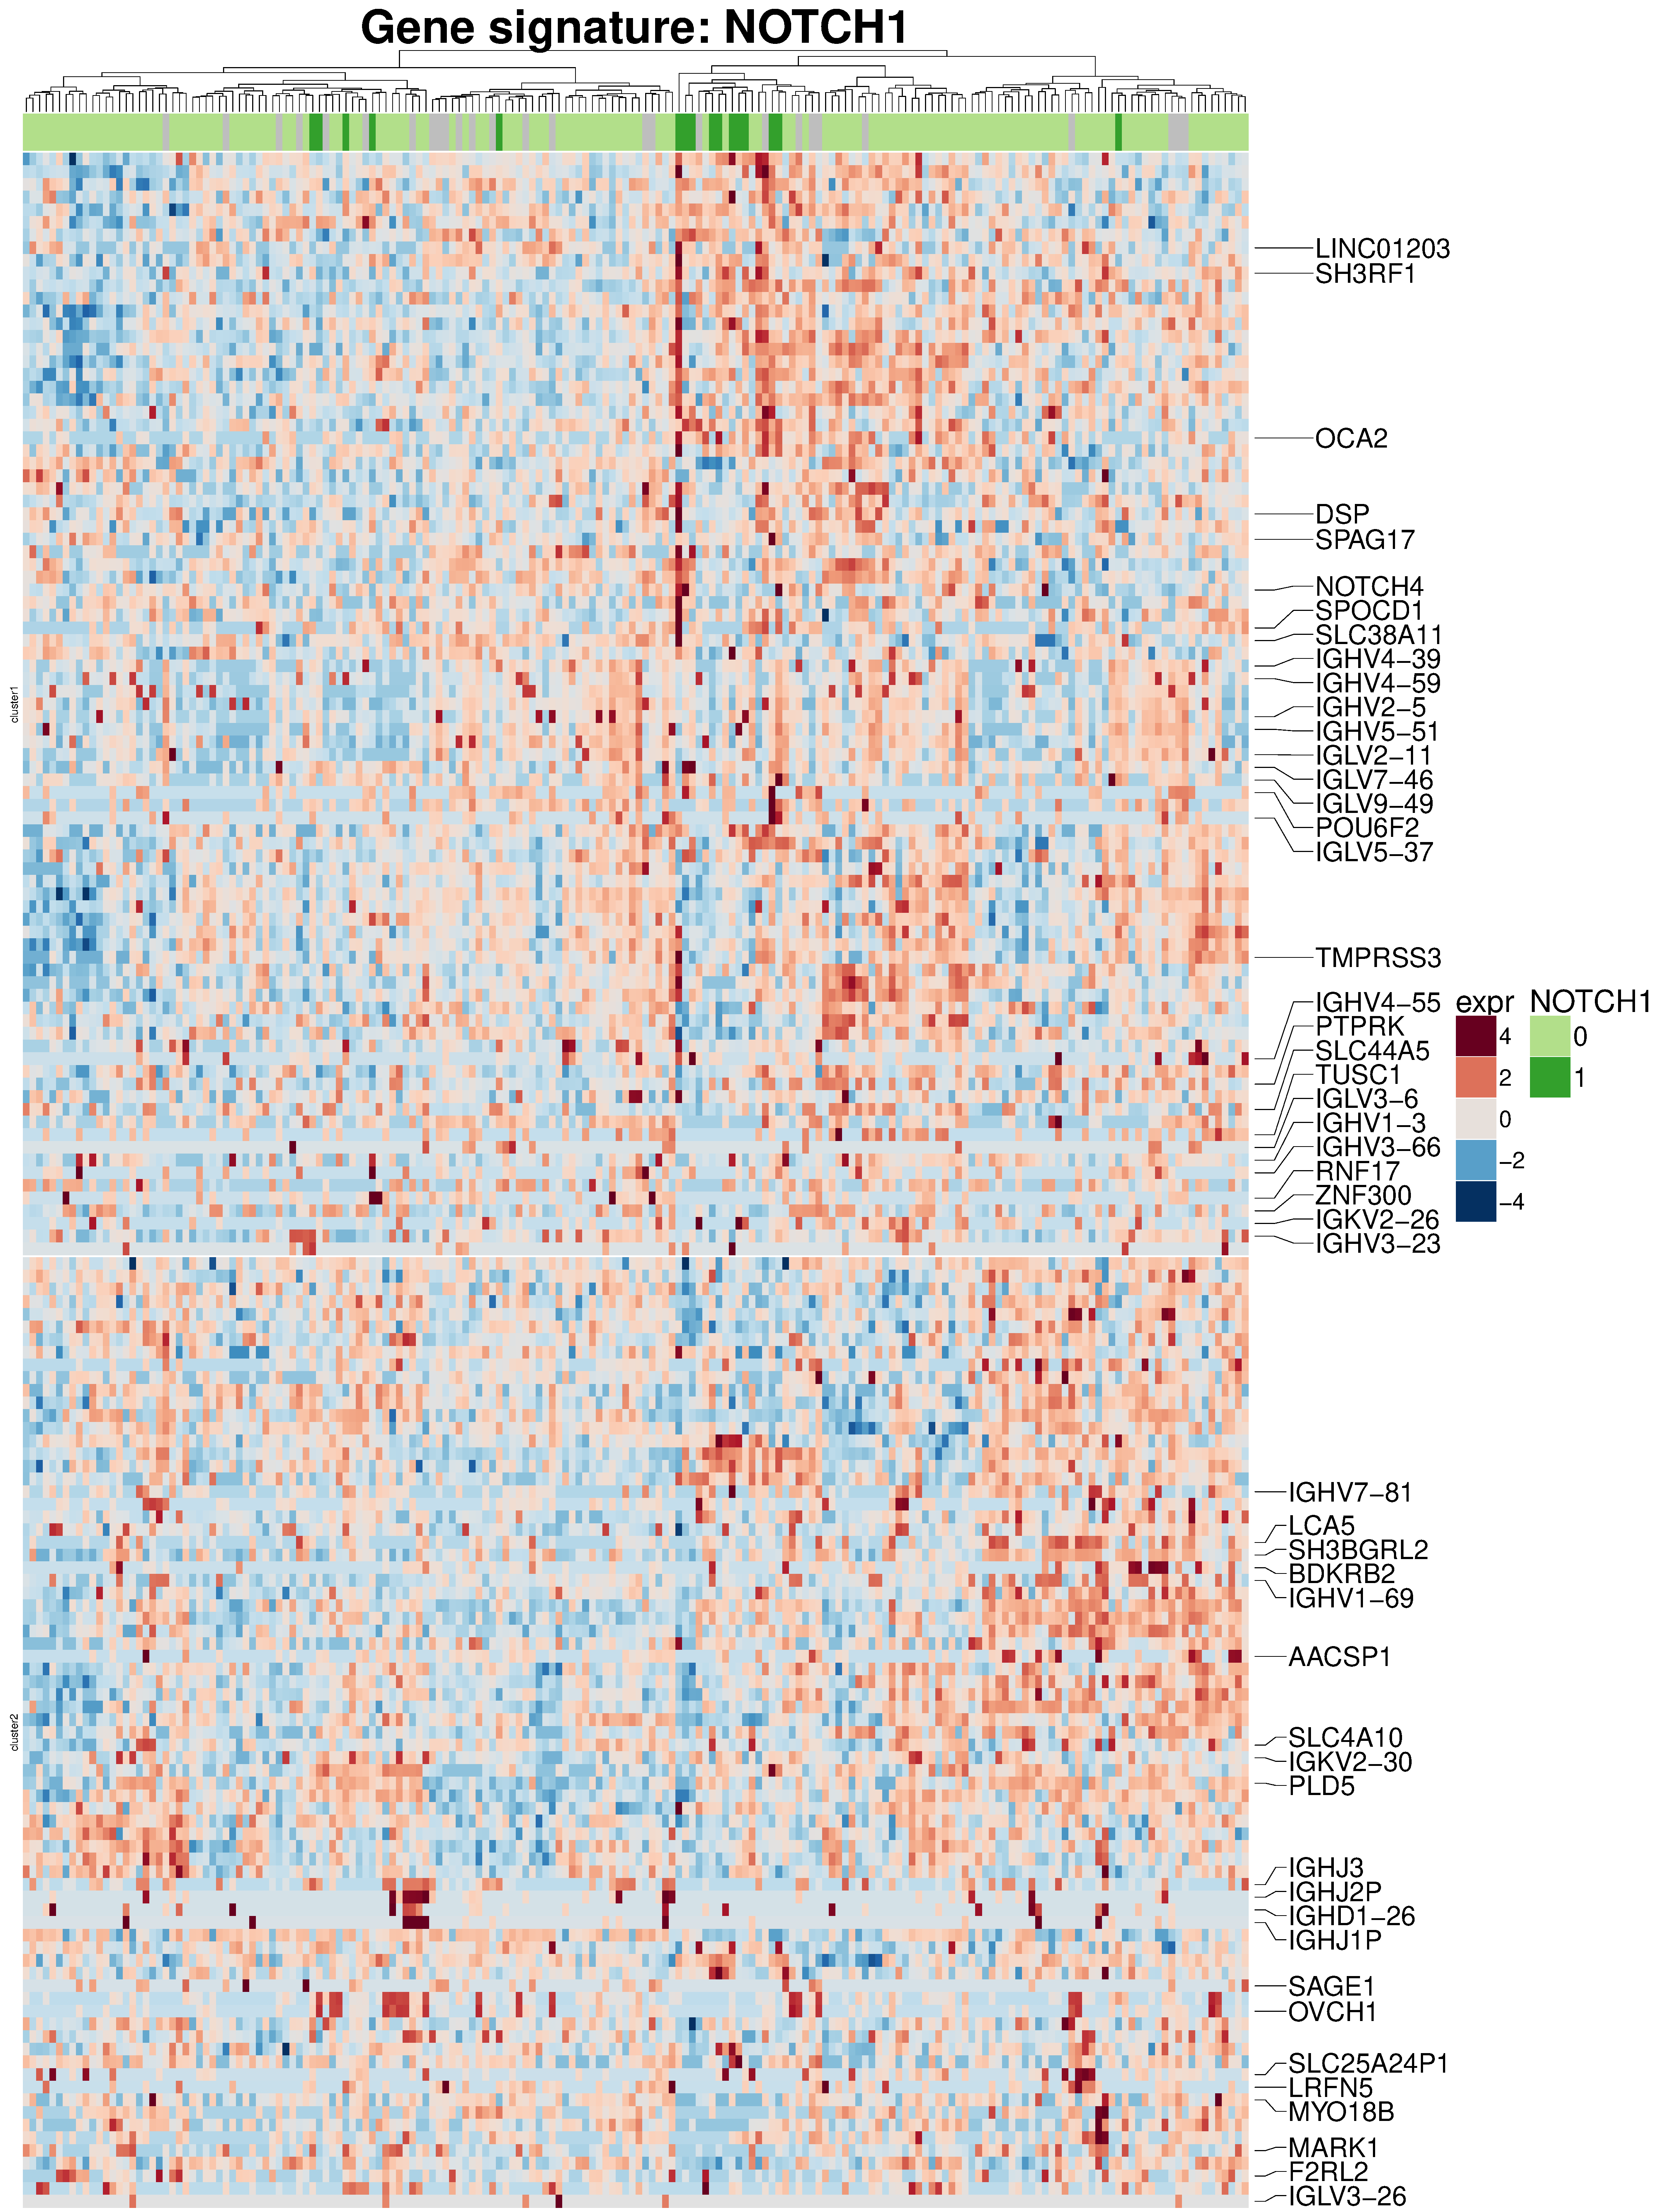
\includegraphics[width=\columnwidth]{./Figures/gene_exprNOTCH1_gsea_Hallmark.pdf}
	\caption{\textbf{Gene expression in Notch1:} Only 162 genes are differentially expressed in Notch1 mutated samples. Notch1 sample do not cluster by them. Annotations show genes from the Kegg Notch signaling pathway. Only Notch4 is differentially expressed.}
	\label{fig:gene_exprNOTCH1_gsea_Hallmark}
\end{figure}

\begin{figure}
	\centering
	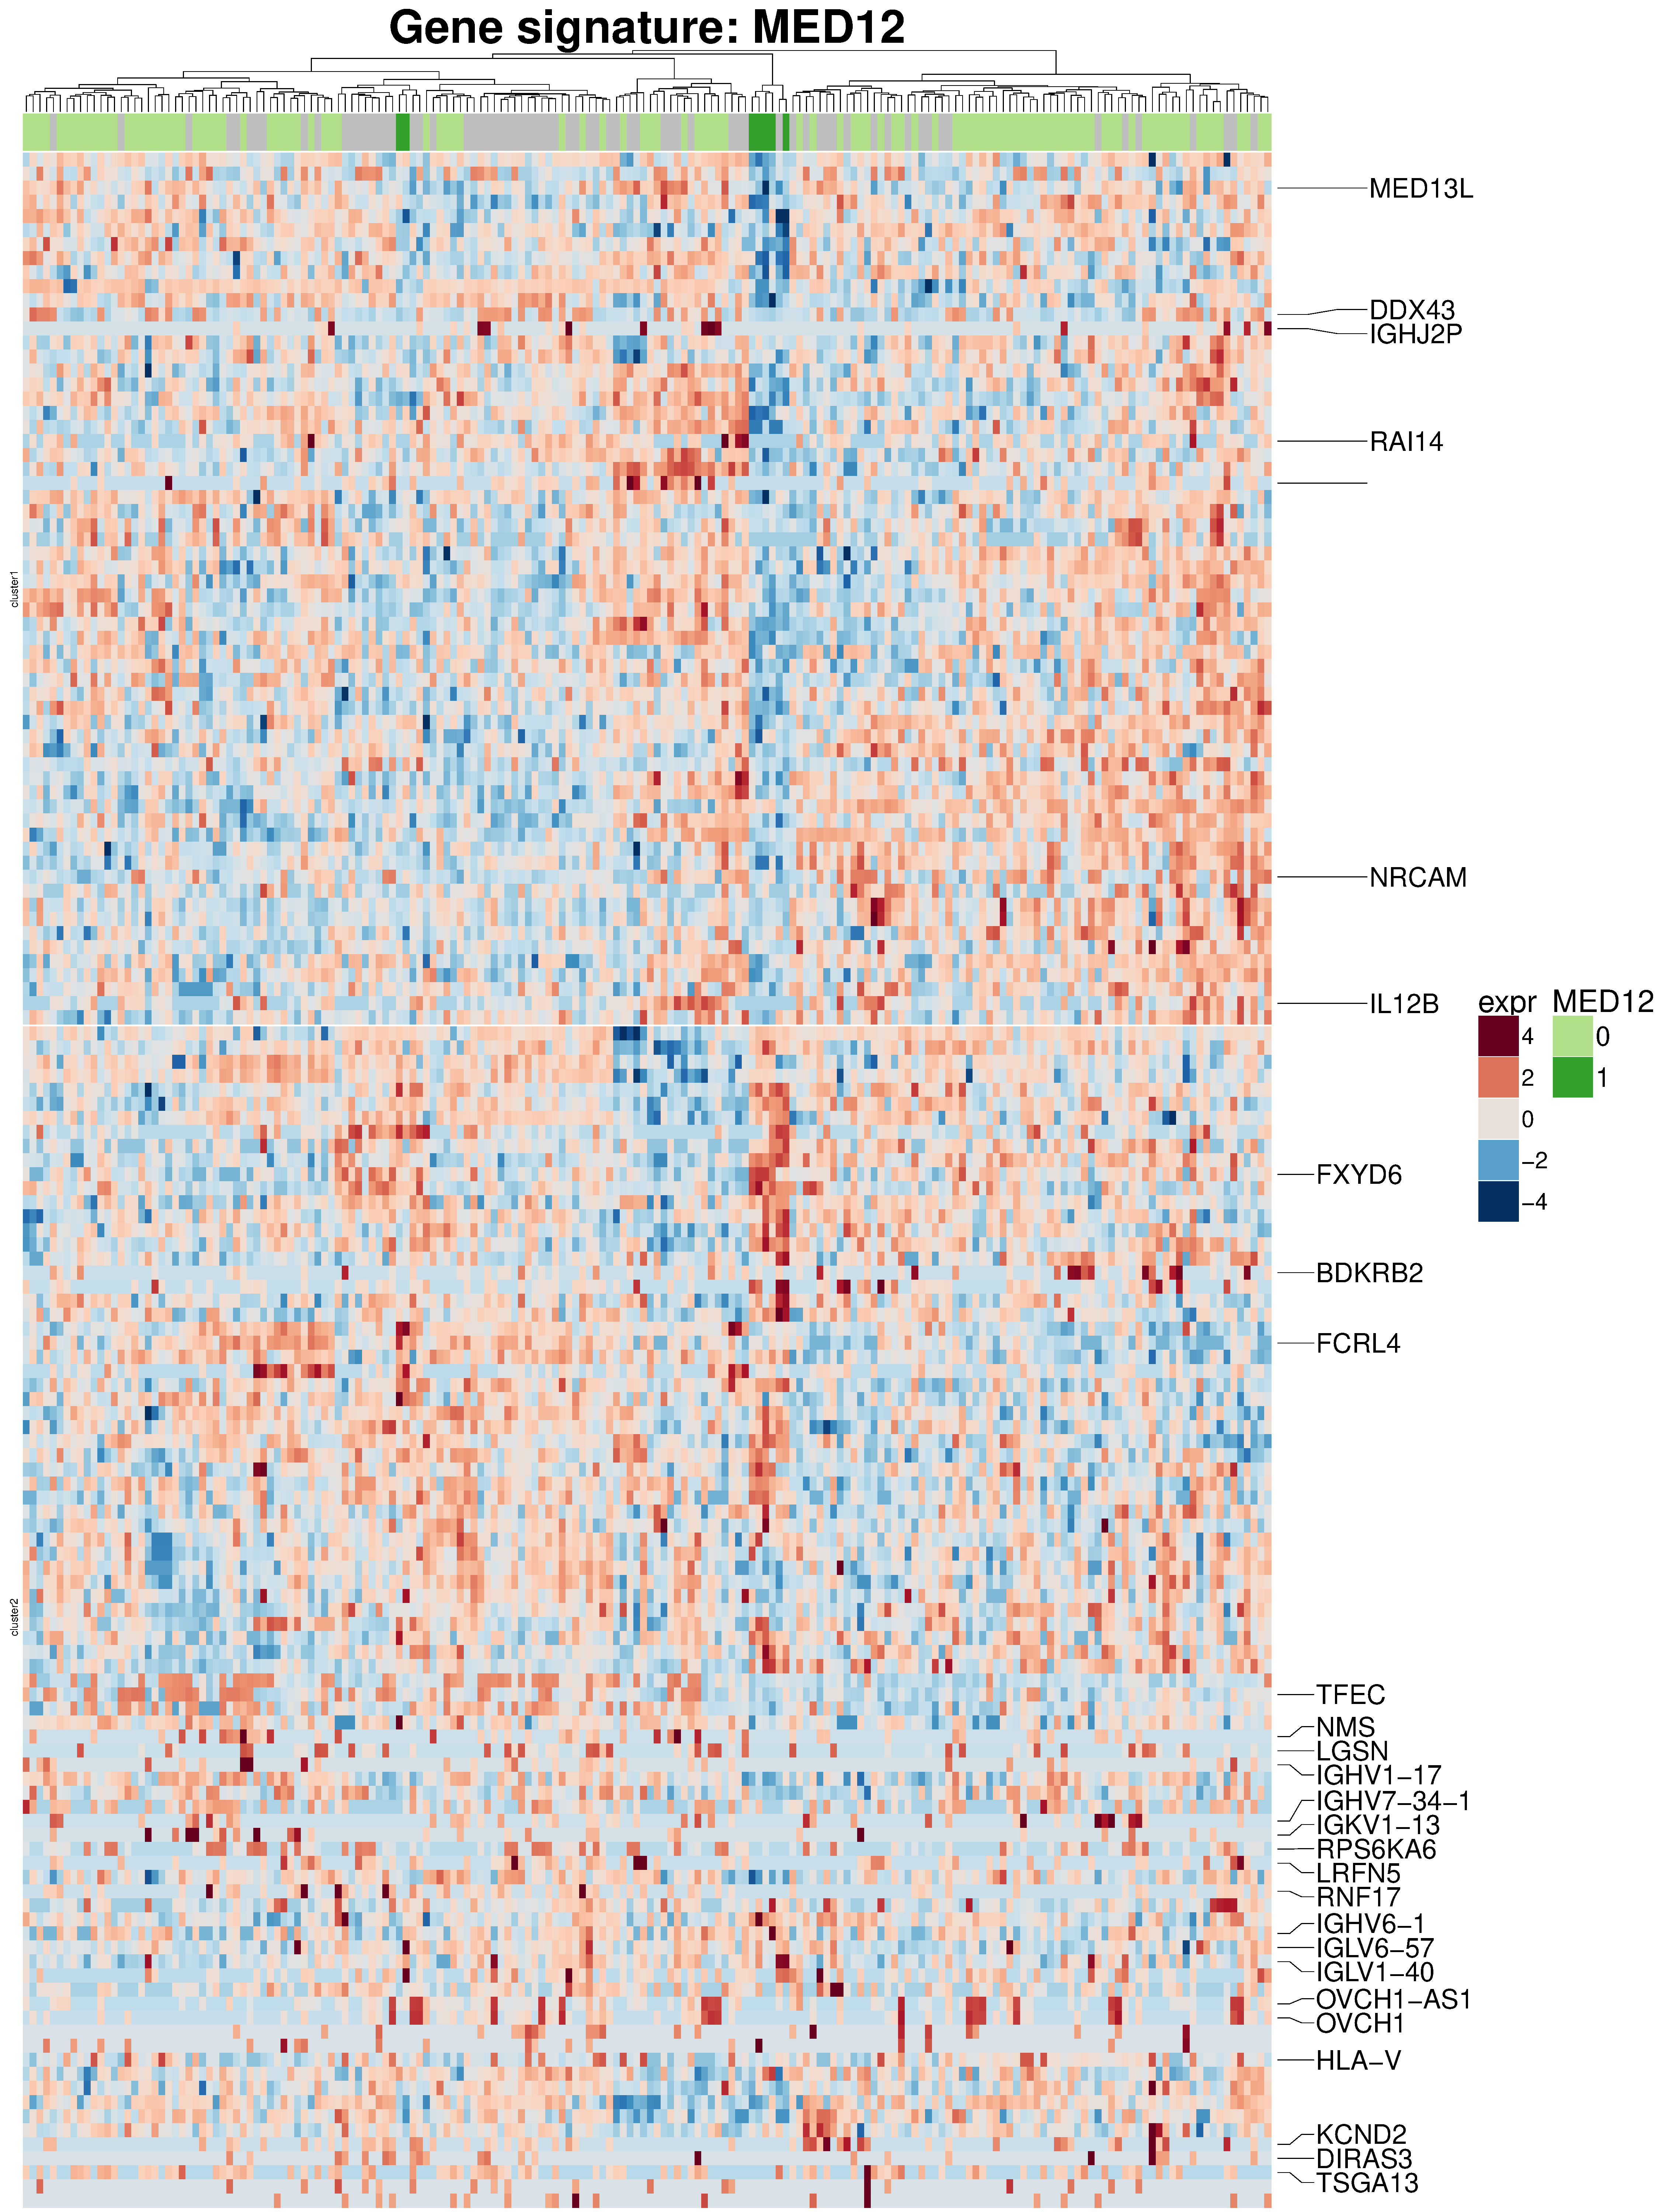
\includegraphics[width=\columnwidth]{./Figures/gene_exprMED12_gsea_Hallmark.pdf}
	\caption{\textbf{Gene expression in MED12:} MED12 mutation has been found in 7 patients. Differential expression analysis reveals significantly different expressed genes in their samples. They do not show distinct pattern, but most MED12 mutated samples cluster by them and MED13L, which is another gene of the mediator complex is among them. Genes with $\log_2$ fold change $>4$ are annotated.}
	\label{fig:gene_exprMED12_gsea_Hallmark}
\end{figure}


\FloatBarrier

\subsection{Enrichment analysis}

\begin{figure}
	\centering
	\begin{subfigure}[t]{0.59\columnwidth}
		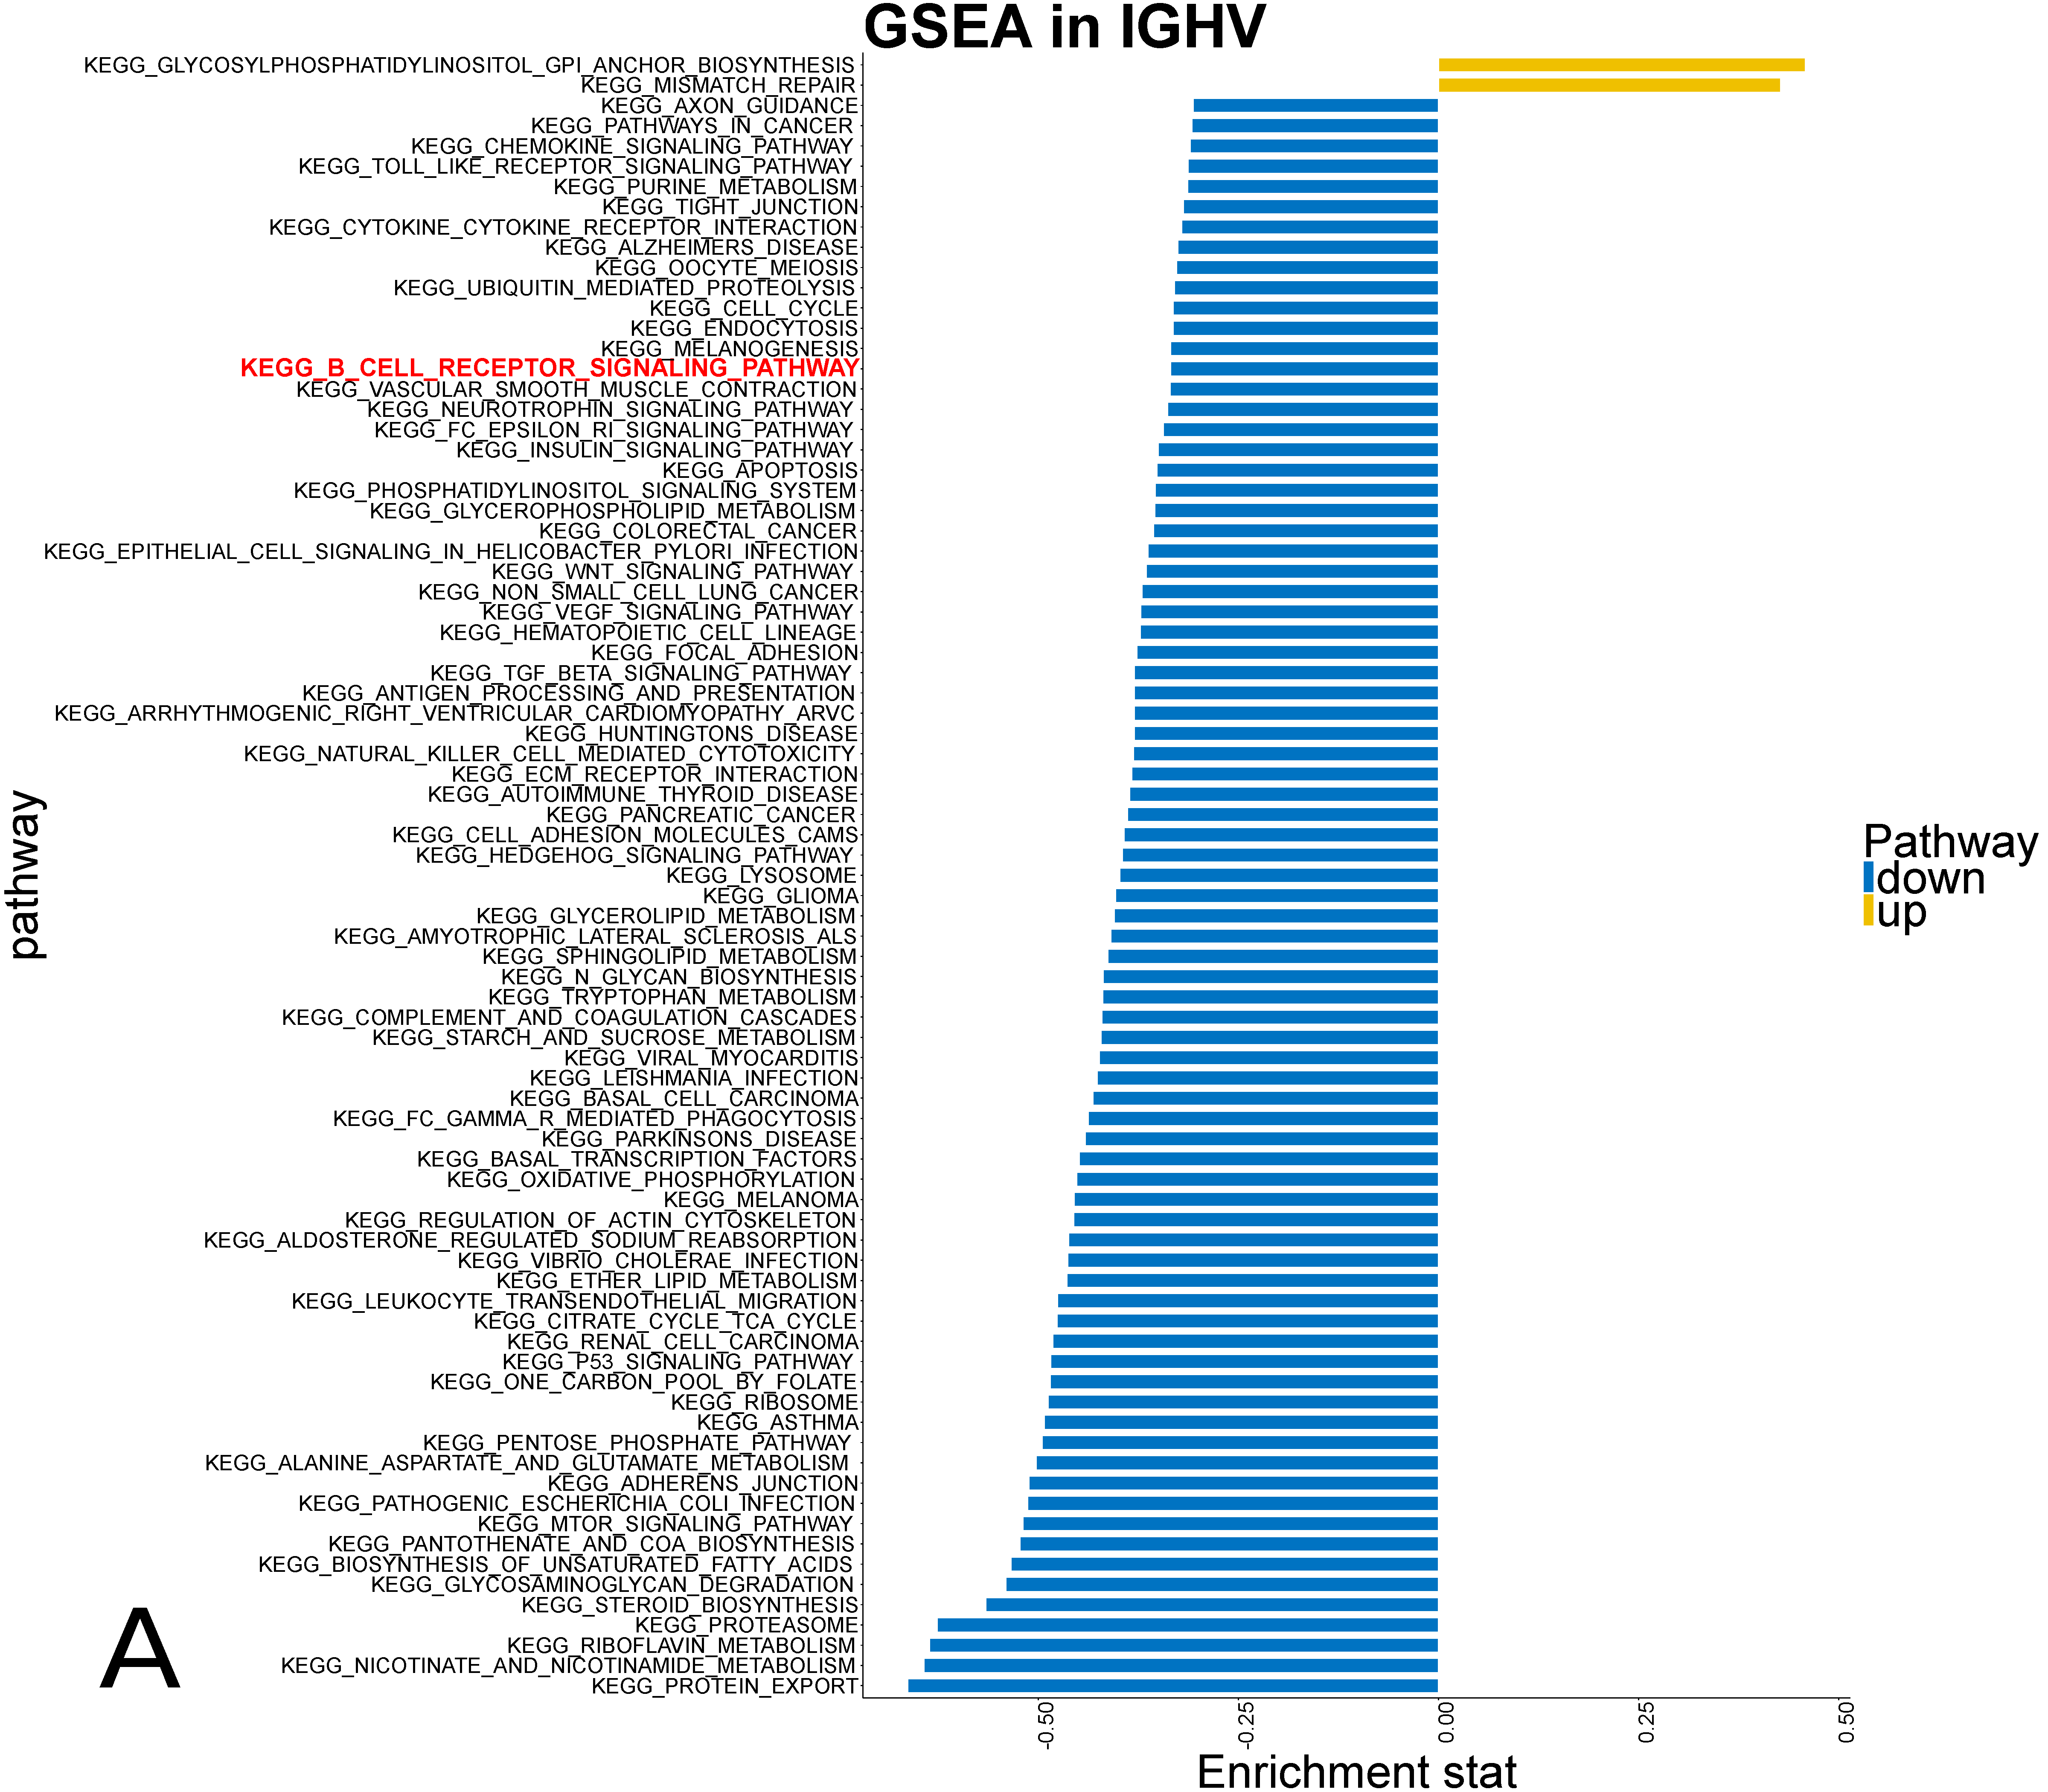
\includegraphics[width=\columnwidth]{./Figures/gseaKegg_IGHV.pdf}
		\subcaption*{}
		\label{fig:gseaKegg_IGHV}
	\end{subfigure}
	\quad
	%add desired spacing between images, e. g. ~,def\svgwidth{\columnwidth} \quad, \qquad, \hfill etc. 
	%(or a blank line to force the subfigure onto a new line)
	\begin{subfigure}[t]{0.33\columnwidth}
		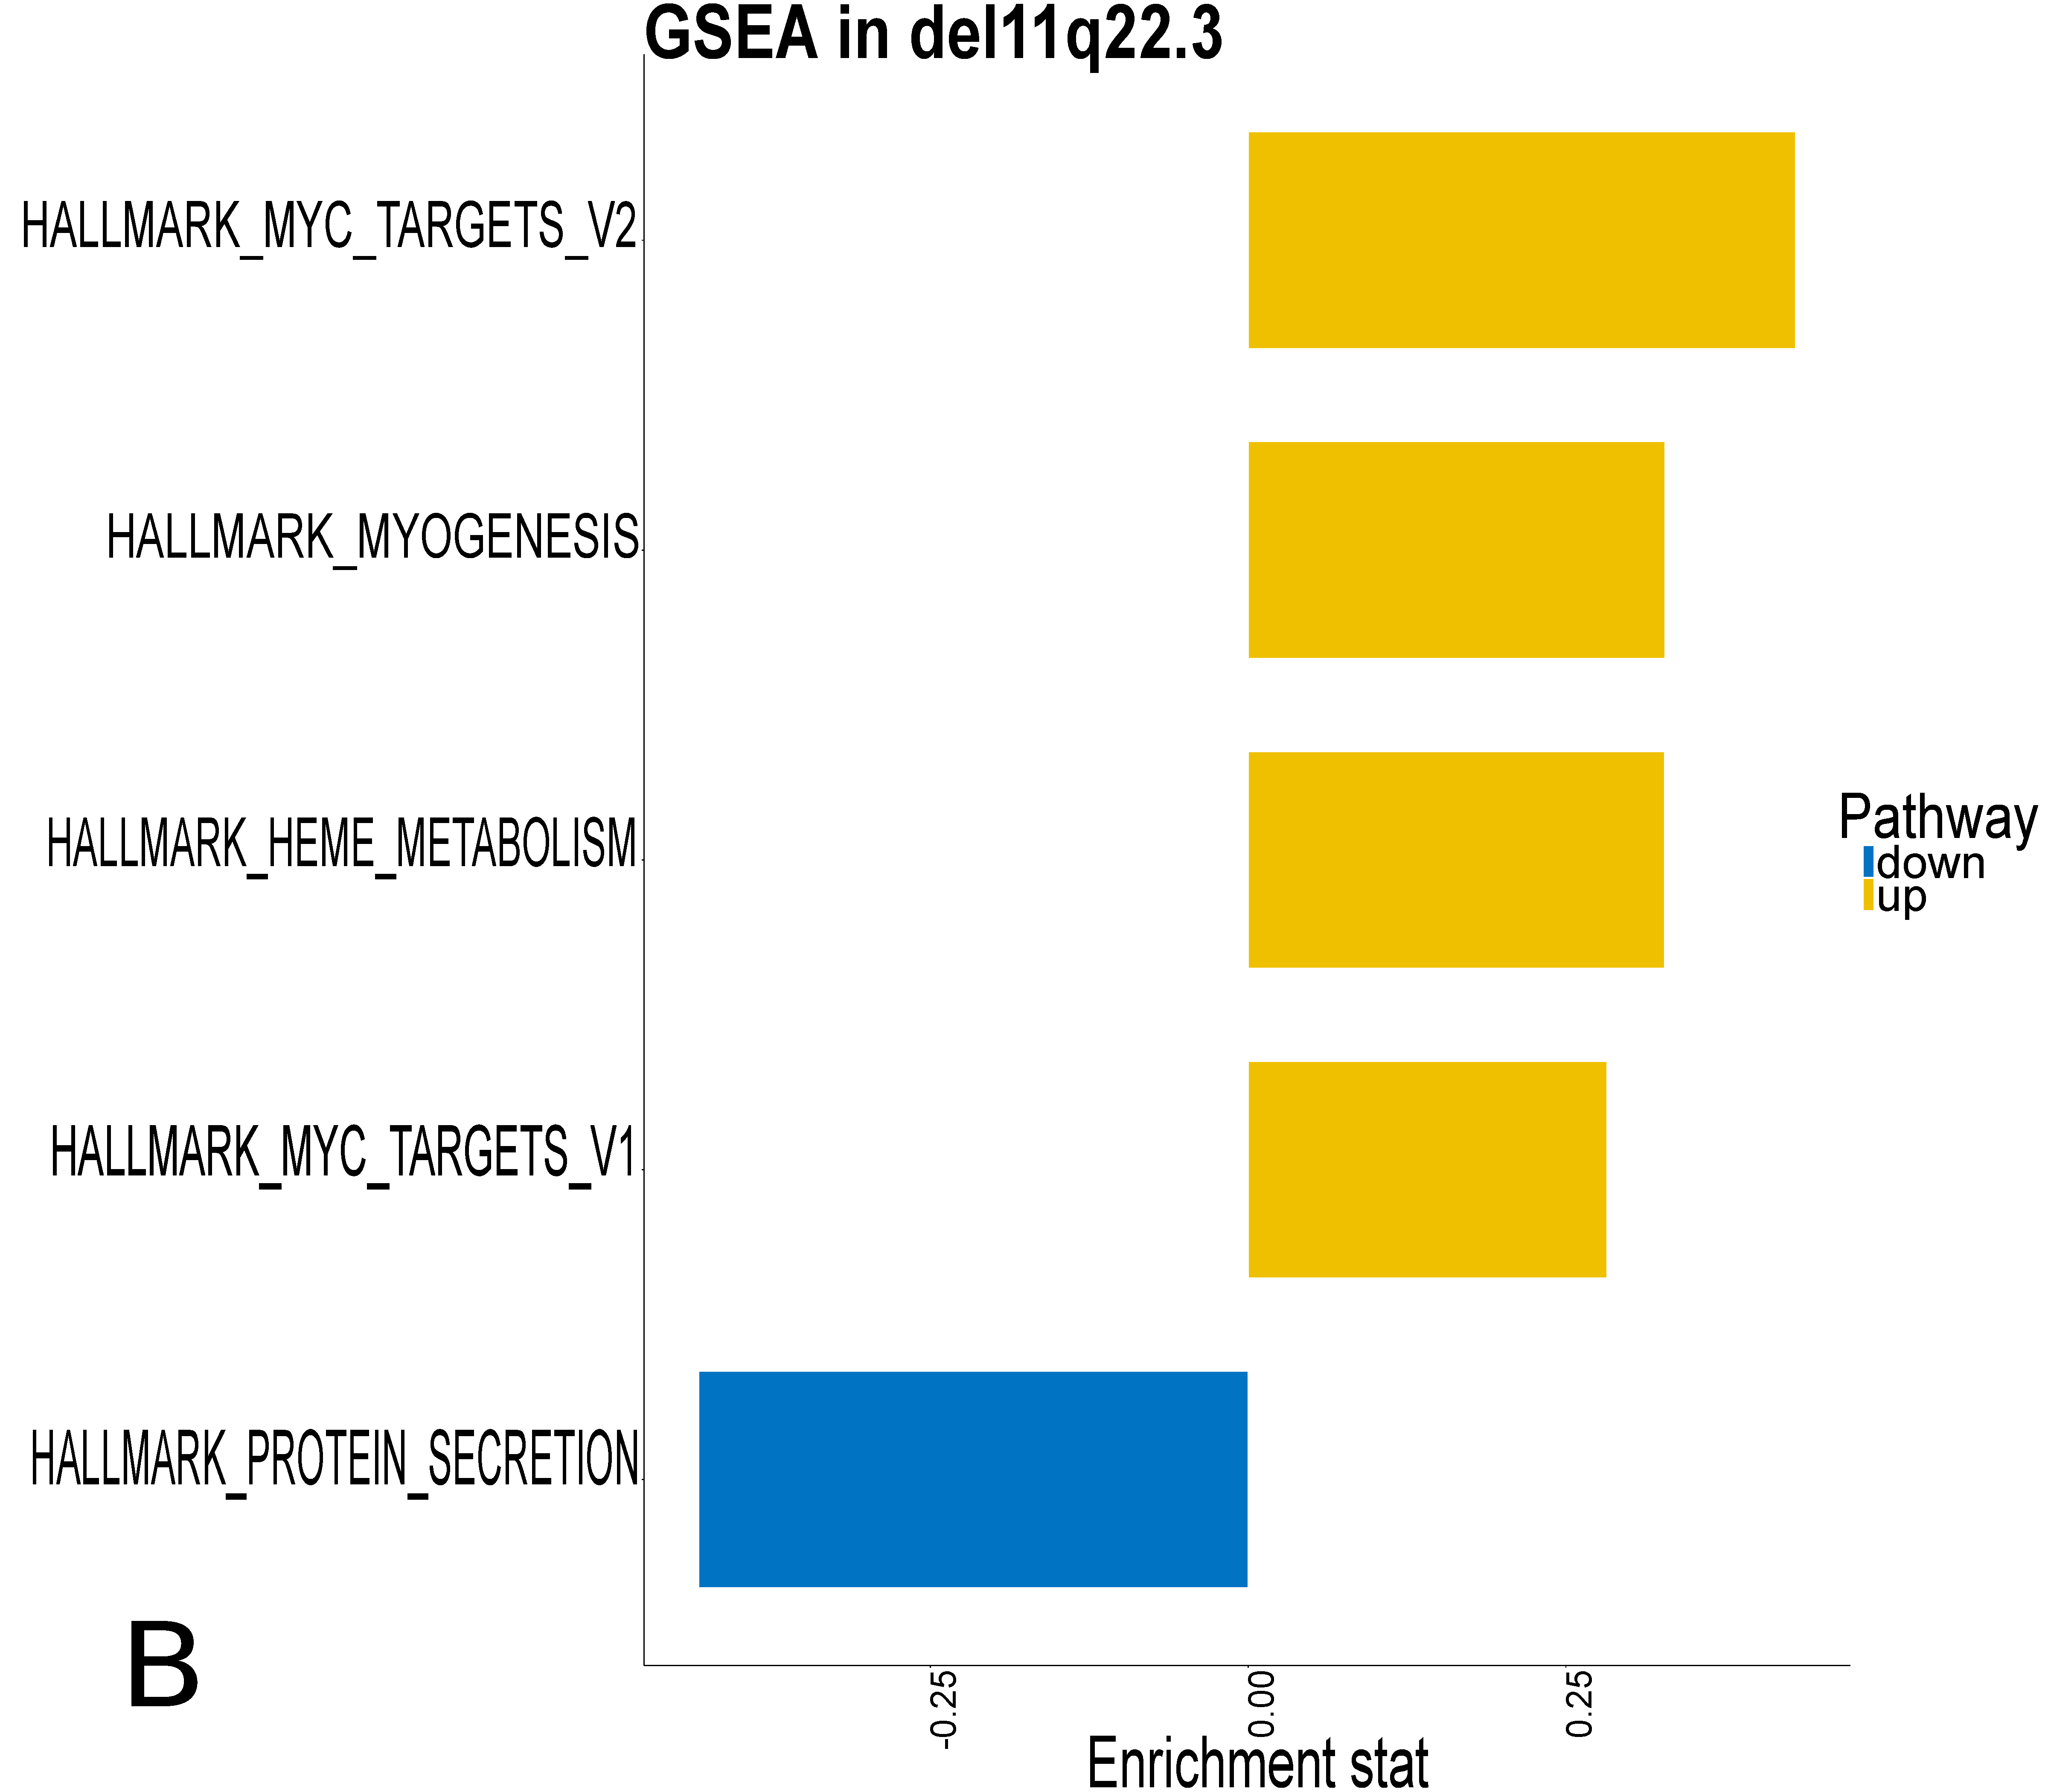
\includegraphics[width=\columnwidth]{./Figures/gseaHallmark_del11.pdf}
		\subcaption*{}
		\label{fig:gsea_del11q22.3}
	\end{subfigure}
	\quad
	\begin{subfigure}[t]{0.47\columnwidth}
		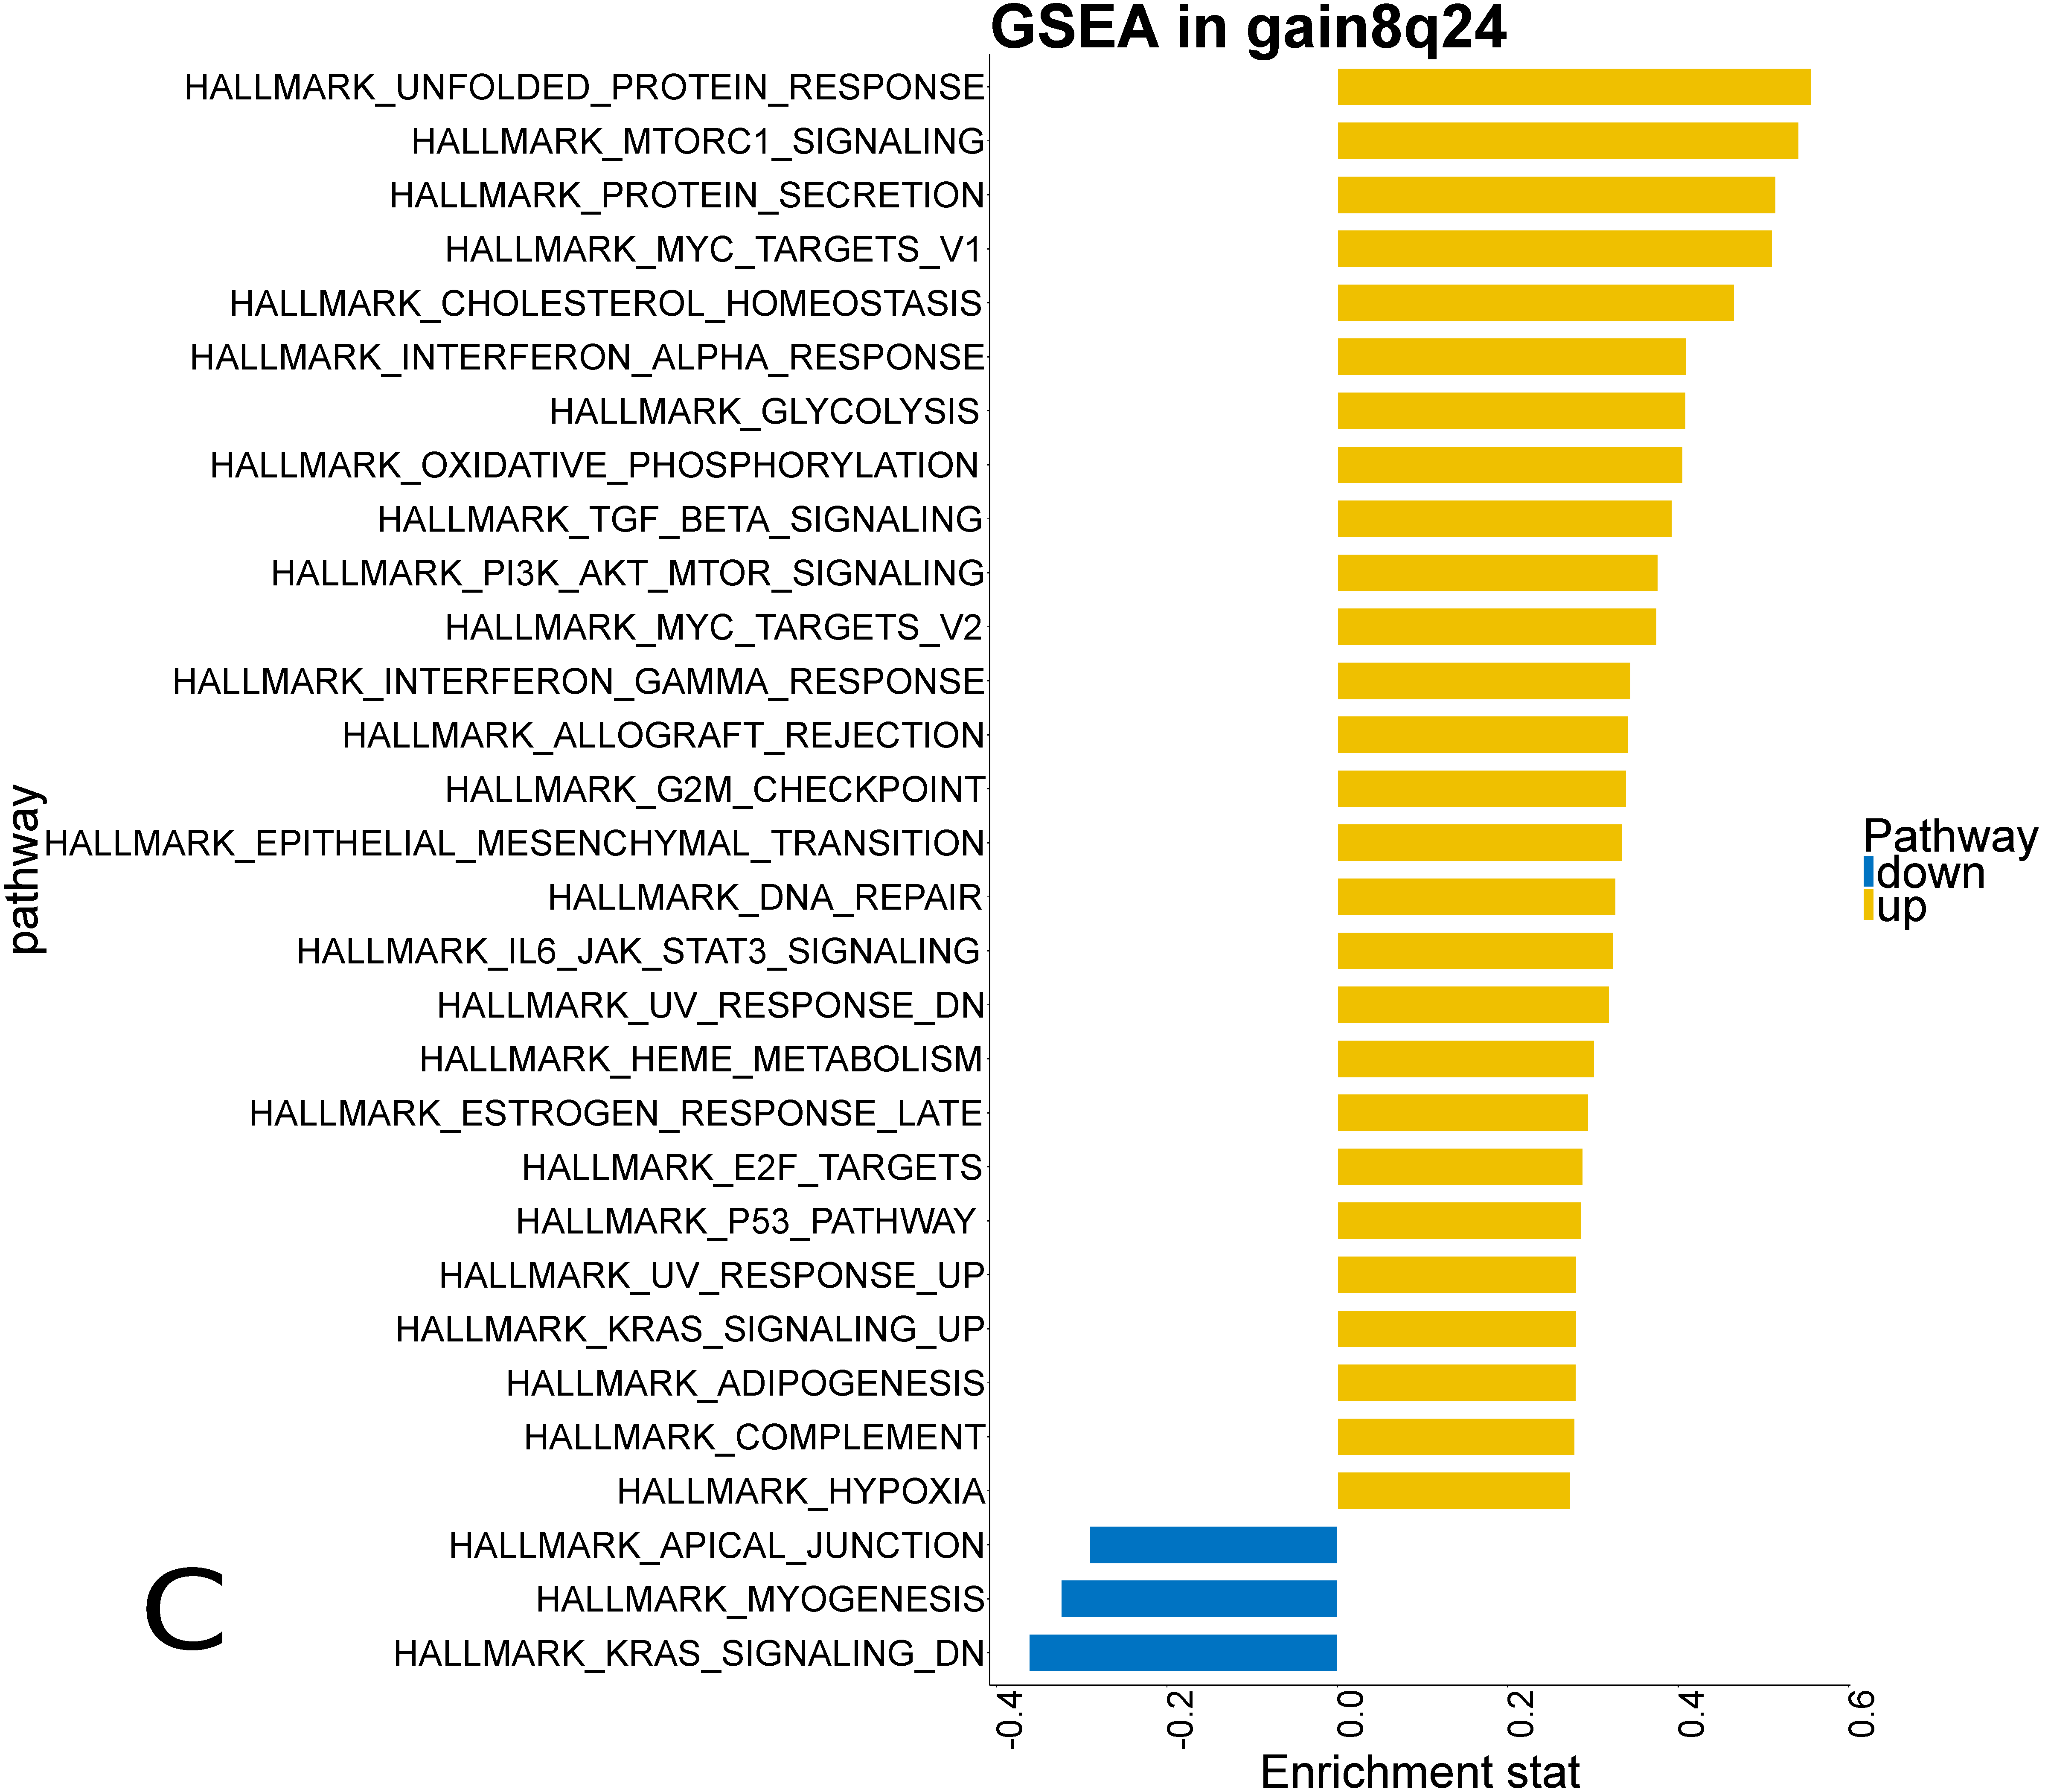
\includegraphics[width=\columnwidth]{./Figures/gseaHallmark_gain8q24.pdf}
		\subcaption*{}
		\label{fig:gsea_gain8q24}
	\end{subfigure}
	\quad
	\begin{subfigure}[t]{0.47\columnwidth}
		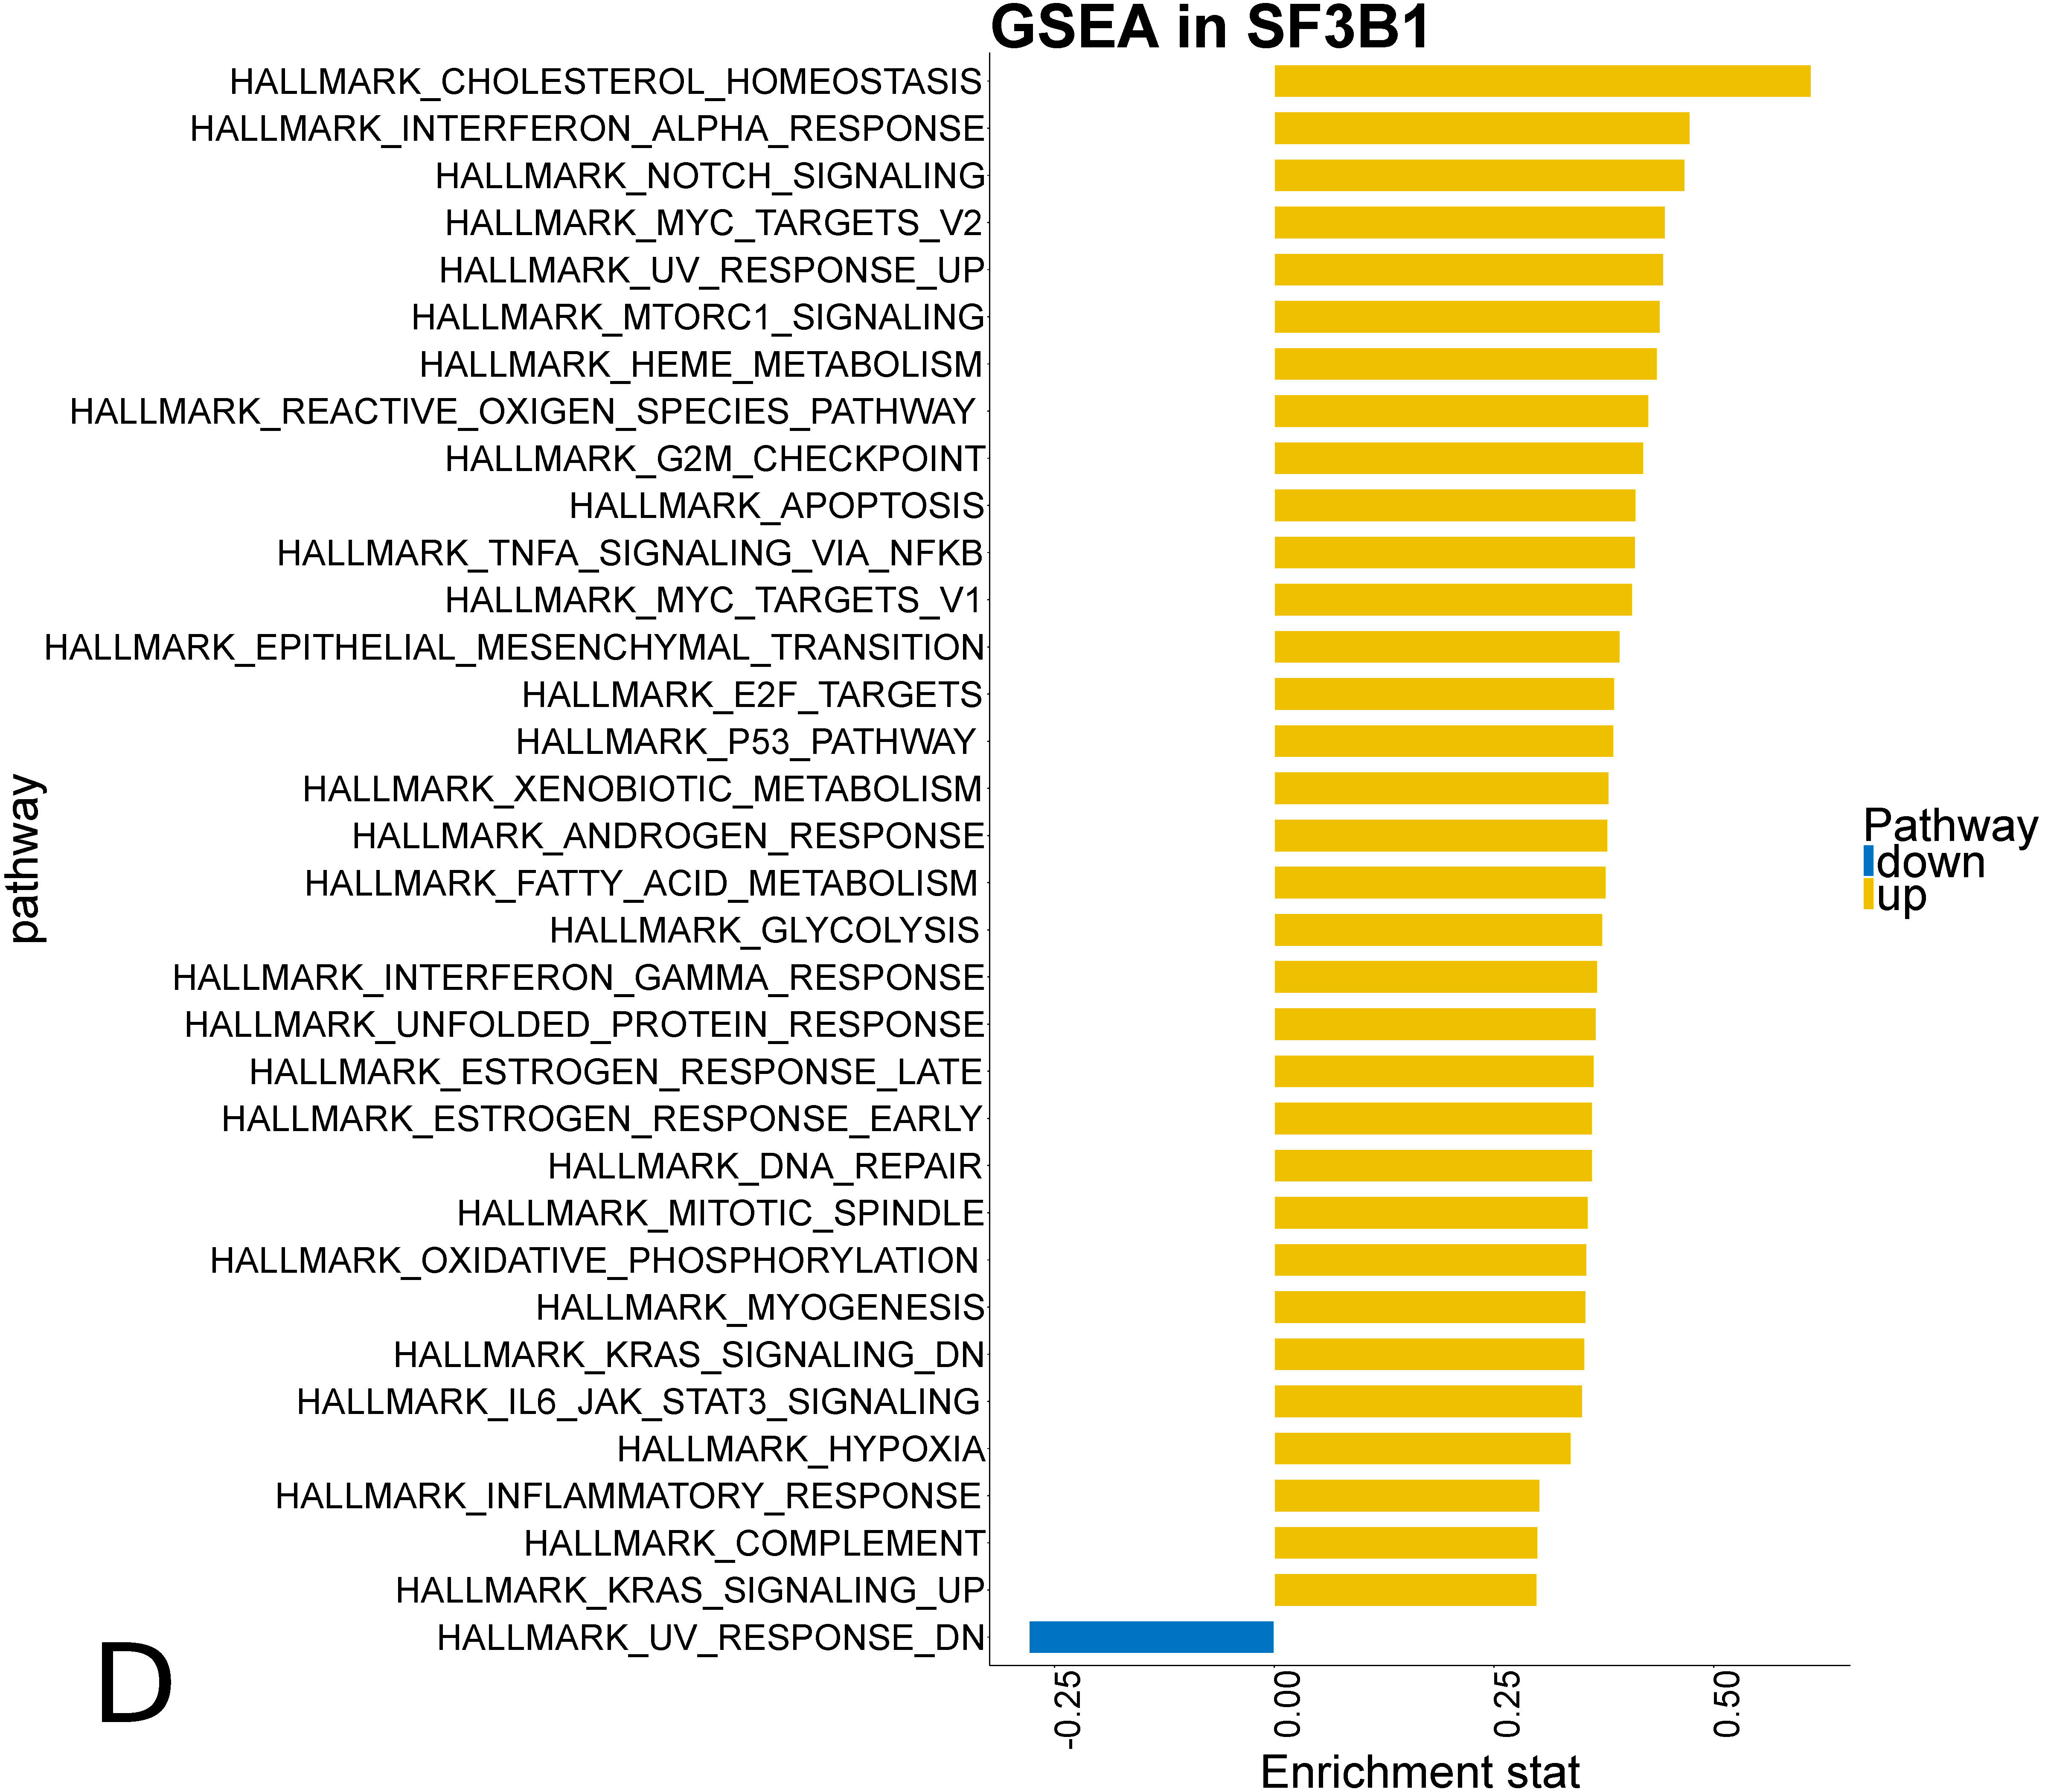
\includegraphics[width=\columnwidth]{./Figures/gseaHallmark_SF3B1.pdf}
		\subcaption*{}
		\label{fig:gsea_SF3B1}
	\end{subfigure}
	\caption{\textbf{Enriched gene sets:} \textbf{(A)} Enriched Kegg pathway in IGHV sample include B cell receptor signaling. It is down regulated in IGHV mutated patients compared to IGHV unmutated patients. \textbf{(B)} Del11q22 samples are up regulated in Myc targets similar to \textbf{(C)} Gain8q24 patients \textbf{(D)} SF3B1 mutation activates many pathways like cholesterol homeostasis, interferon alpha signaling and Notch signaling pathway.}
	\label{fig:Enrichment_others}
	
\end{figure}


\FloatBarrier